\documentclass{IEEEconf}
\usepackage{graphicx}
\usepackage{hyperref}
\usepackage{algorithm}
\usepackage{amsmath}
\usepackage{algpseudocode}
\usepackage{color, colortbl}
\usepackage{multicol}
\definecolor{LightYellow}{rgb}{1, 0.9, 0.78}

\title{\textbf{GPU Computing} \\
    \large Homework 2: Matrix Transposition \\
}
\author{Murtas Cristian \\ 248025 \\ cristian.murtas@studenti.unitn.it \\
\underline{\href{https://github.com/SecondarySkyler/gpu-computing/tree/main/cuda_matrix_transposition}{GitHub Repository}}
} 

\begin{document}
\maketitle
\begin{abstract}
    This work focuses on the implementation of different algorithms for matrix transposition on the CPU and on the GPU.
    First, a formal definition of the problem is provided and followed by the description of the pseudocodes.
    On the CPU side the performance of the algorithms has been evaluated using different optimization flags, while the GPU side has been evaluated using different kernel configurations.
    Through the experiments, the performance of the algorithms has been evaluated. In particular, the attention has been put on diverse metrics
    such as the effective bandwidth and the cache behavior (for the CPU case).
    In the end, the results have been analyzed and discussed.
\end{abstract}
\section{Problem Description}
The goal of this homework is to implement a matrix transposition algorithm, where the transpose of a matrix $A$
is an operation that flips $A$ over its diagonal. 
If $A$ is of size $m \times n$ and $e$ is the element at row $i$ and column $j$, then the transpose of $A$ - also denoted as $A\textsuperscript{T}$ - 
is a matrix of size $n \times m$, where $e$ is at row $j$ and column $i$.  \\
Additionally, we are asked to measure the effective bandwidth of our implementation, also considering  the
usage of different optimization flags, such as: \texttt{-O0}, \texttt{-O1}, \texttt{-O2}, \texttt{-O3}.
Furthermore, an analysis of the cache behavior related to the algorithm is required and, for this purpose, we are going to use
valgrind.
\subsection{Algorithms}
Two algorithms have been implemented. The first one is a na\"{i}ve approach, which
consists in iterating over the $src$ matrix, reading the data at position $src[i][j]$ and writing it at position $dest [j][i]$. The second algorithm is a more optimized version, which takes advantage of a block mechanism to reduce the number of cache misses.
\begin{algorithm}
    \caption{Na\"{i}ve Matrix Transposition}
    \begin{algorithmic}[1]
        \State $src \gets create\_matrix(size)$
        \For{$i = 0$ to $size$}
            \For{$j = 0$ to $size$}
                \State $dest[j * size + i] = src[i * size + j]$
            \EndFor
        \EndFor
    \end{algorithmic}
\end{algorithm}
\begin{algorithm}
    \caption{Matrix Transposition with Blocking}
    \begin{algorithmic}[1]
        \State $src \gets create\_matrix(size)$
        \For{$i = 0$ to $size$ increase $i$ by $block\_size$}
            \For{$j = 0$ to $size$ increase $j$ by $block\_size$}
                \For{$k = i$ to $i$ + $block\_size$} \Comment{Loop over the current block}
                    \For{$l = j$ to $j$ + $block\_size$}
                        \State $dest[l * size + k] = src[k * size + l]$
                    \EndFor
                \EndFor
            \EndFor
        \EndFor
    \end{algorithmic}
\end{algorithm}
\section{Experimental Setup}
\subsection{Hardware} \label{hardware}
The entire experiment has been conducted on the Marzola cluster of the University of Trento, 
which has an Intel Xeon Silver 4309y \cite{intel:xeon} and NVIDIA A30 GPUs \cite{nvidia:a30}.
The code has also been tested on a local machine equipped with an AMD Ryzen 5 5600X 
\cite{amd:ryzen} and an NVIDIA RTX 3070 \cite{nvidia:rtx3070}.
For both setup, the information about the GPUs have been retrieved using the 
\textit{cudaGetDeviceProperties} function \cite{nvidia:cudaDeviceProp}.
\subsection{Results}
To provide a broader and precise analysis, the results have been collected executing both algorithms on matrices of different sizes,
ranging from $4 \times 4$ to $4096 \times 4096$. Also, for each dimension, the algorithms have been executed multiple times (100) to further improve the measurements. \\
The effective bandwidth has been calculated using the formula below: \\
\begin{equation*}
    Effective \: Bandwidth = \frac{\left ( \textit{2} * dimension * dimension * \textit{4} \right )}{execution\: time}
    \left[\frac{GB}{s}\right]
\end{equation*}
The factor \textit{2} is because we are both reading and writing the matrix; the $dimension$ is the size of the matrix; 
\textit{4} is the size of a single floating element in bytes and the $execution \: time$ is the average time of the 100 executions. \\
\subsubsection{Na\"{i}ve Algorithm}
The obtained results are in line with the expectations. Indeed, the executions with \texttt{-O0} don't show any significant difference because the compiler 
doesn't apply any optimization. Meanwhile, the executions with \texttt{-O1}, \texttt{-O2} and \texttt{-O3} show a significant improvement in the performance, on all
the tested platforms. This is probably due to the fact that the compiler is able to apply some optimizations, such as loop unrolling. \\
Another interesting aspect is that both the Ryzen 5 and the Xeon start to show a decrease in the performance when the matrix size is greater than $64 \times 64$, 
as shown in figure \ref{fig:naive_comparison}. \\
To understand this behavior, the cache miss rate has been analyzed using valgrind (table \ref{tab:naive_cache_miss}). \\ 
\begin{table}[h]
    \centering
    \begin{tabular}{|c|c|c|}
        \hline
        \multicolumn{3}{|c|}{\textbf{Ryzen 5 5600X}} \\
        \hline
        \textbf{Dimension}            & \textbf{I1 miss rate} & \textbf{D1 miss rate} \\ \hline
        64                   & 0.01\%       & 0.4\%        \\ \hline
        128                  & 0.00\%       & 4.0\%        \\ \hline 
    \end{tabular}
    \hspace{2em}
    \begin{tabular}{|c|c|c|}
        \hline
        \multicolumn{3}{|c|}{\textbf{Xeon 4309y}} \\
        \hline
        \textbf{Dimension}            & \textbf{I1 miss rate} & \textbf{D1 miss rate} \\ \hline
        64                   & 0.01\%       & 0.1\%        \\ \hline
        128                  & 0.00\%       & 3.6\%        \\ \hline 
    \end{tabular}
    \caption{Cache miss rate of the na\"{i}ve algorithm}
    \label{tab:naive_cache_miss}
\end{table}
\begin{figure*}
    \centering
    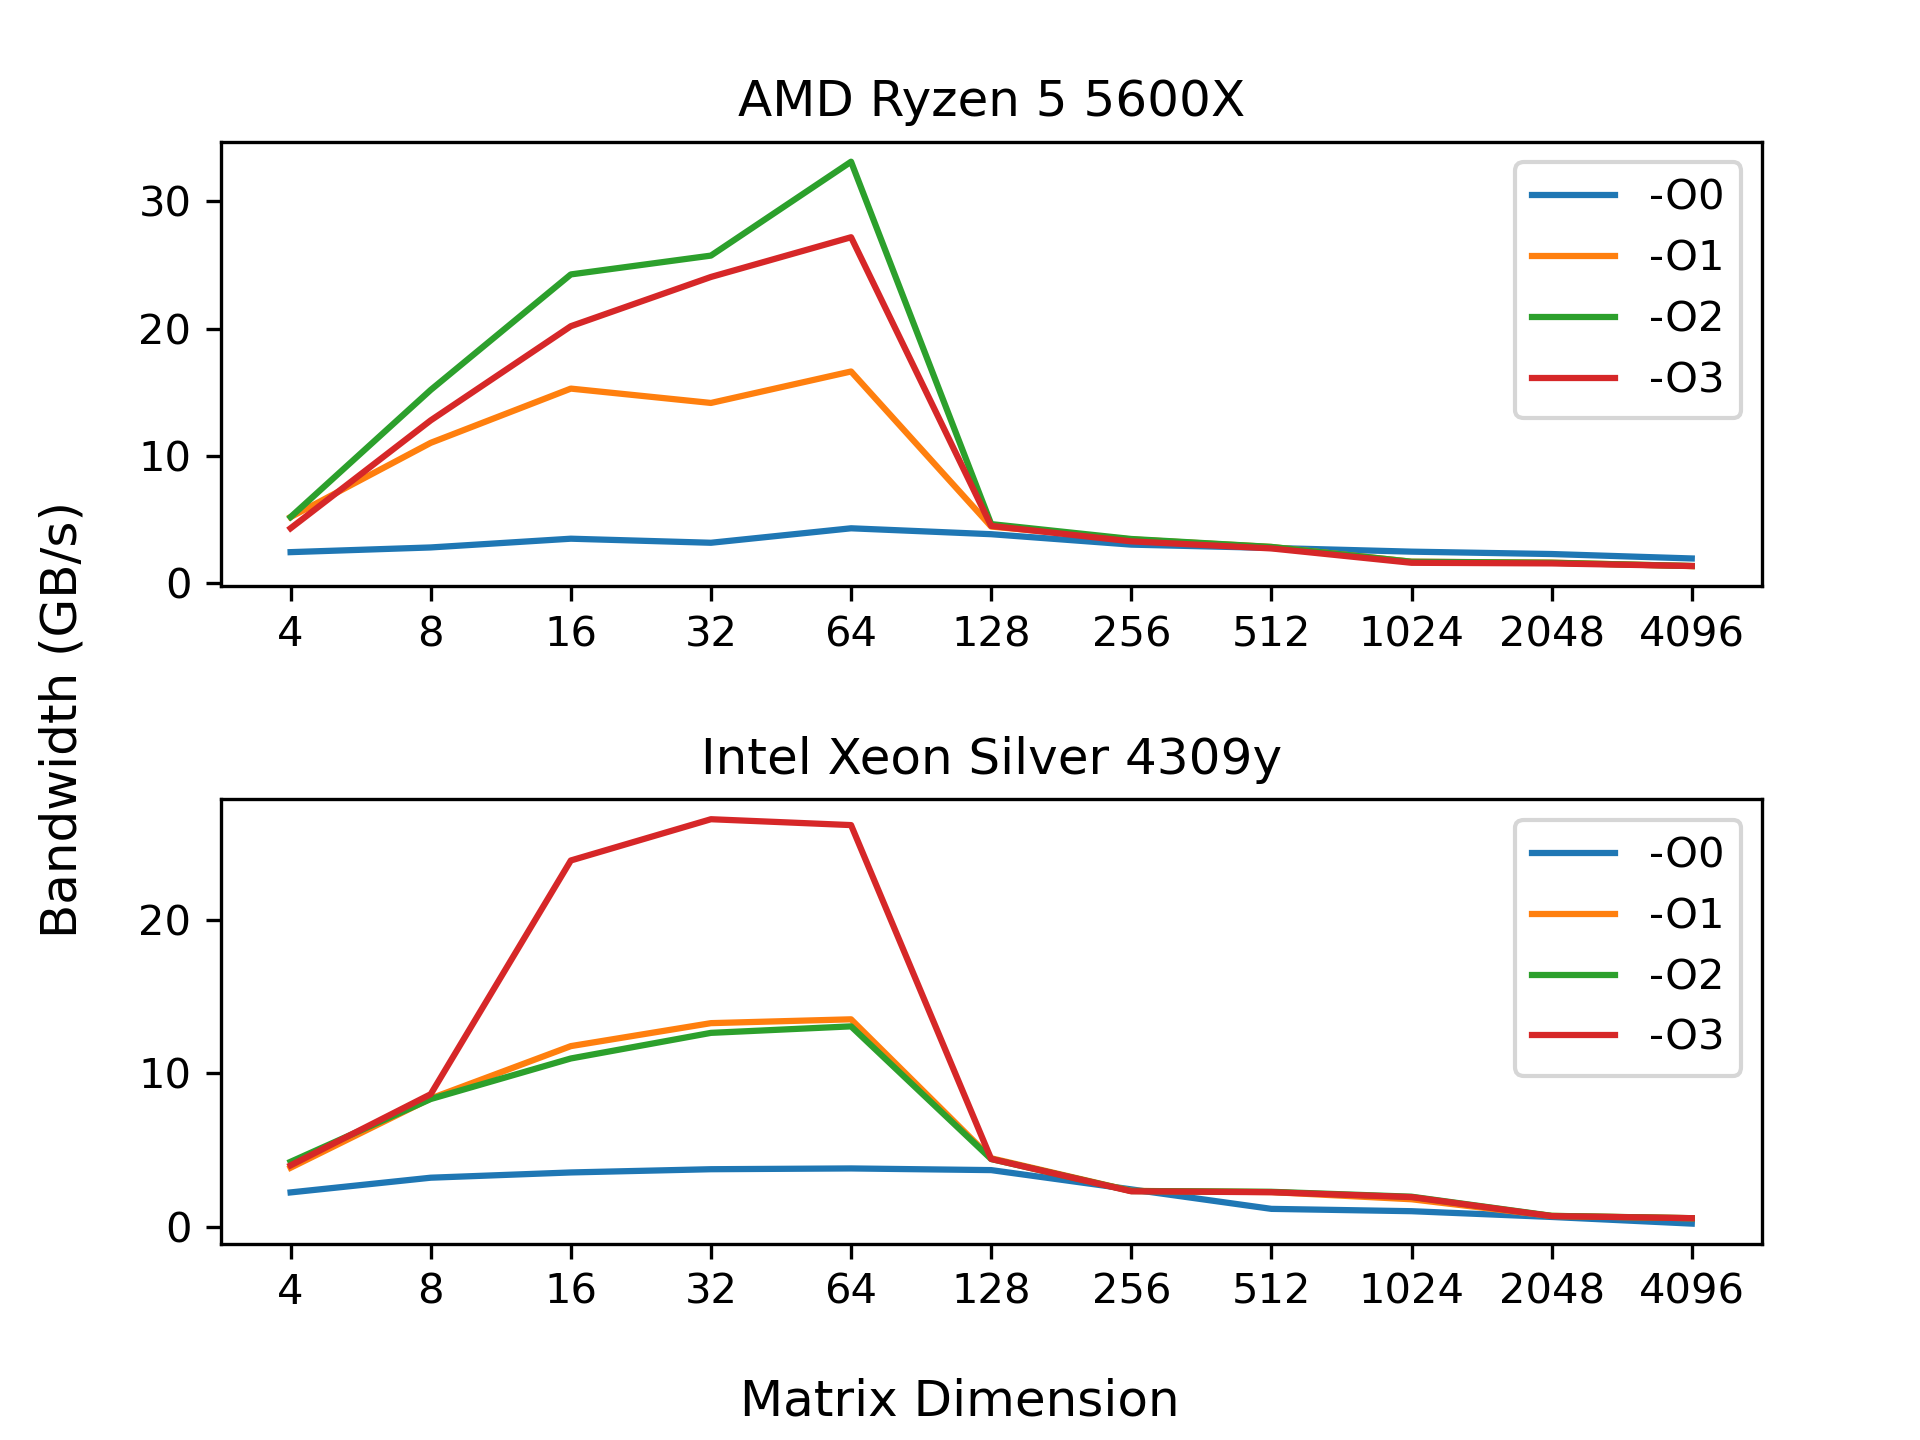
\includegraphics[scale=0.8]{report/img/naive_comparison.png}
    \caption{Comparison of the na\"{i}ve matrix transposition algorithm}
    \label{fig:naive_comparison}
\end{figure*}
\subsubsection{Blocked Algorithm}
The idea behind the blocked algorithm is to reduce the number of cache misses by exploiting the locality of the data. But in order to benefit from this the block
size must be chosen with care, since it also depends on the size of the cache line. Different dimensions have been used to test the algorithm and find the best one.
In this step, we used a matrix of $1024 \times 1024$ and set the optimization flag to \texttt{-O3}.
The results for the used platforms are shown in table \ref{tab:blocked_results}, where the highlighted rows indicate the most appropriate 
block size for the given processor. \\
Subsequently, as shown in figure \ref{fig:blocked_comparison}, the results are pretty evident. Indeed, the blocked algorithm outperforms the na\"{i}ve one on both platforms. \\
The cache miss rate analysis highlights how the blocked algorithm is able to exploit the temporal locality of the data.
The results of the analysis are shown in table \ref{tab:blocked_cache_miss}. \\

\begin{table}[h]
    \centering
    \begin{tabular}{|c|c|}
        \hline
        \multicolumn{2}{|c|}{\textbf{Ryzen 5 5600X}} \\
        \hline
        \textbf{Blocksize } & \textbf{Bandwidth (GB/s)} \\ \hline
        2         & 4.85 \\ \hline
        \rowcolor{LightYellow}
        4         & 7.49 \\ \hline
        8         & 3.47 \\ \hline
        16        & 3.62 \\ \hline
        32        & 3.33 \\ \hline
        64        & 2.75 \\ \hline
    \end{tabular}
    \hspace{2em}
    \begin{tabular}{|c|c|}
        \hline
        \multicolumn{2}{|c|}{\textbf{Xeon 4309y}} \\
        \hline
        \textbf{Blocksize } & \textbf{Bandwidth (GB/s)} \\ \hline
        2         & 2.04 \\ \hline
        4         & 3.83 \\ \hline
        \rowcolor{LightYellow}
        8         & 4.80 \\ \hline
        16        & 2.45 \\ \hline
        32        & 2.59 \\ \hline
        64        & 2.72 \\ \hline
    \end{tabular}
    \caption{Results of the blocked algorithm with different block sizes ($1024 \times 1024$, \texttt{-O3})}
    \label{tab:blocked_results}
\end{table}
\begin{figure*}
    \centering
    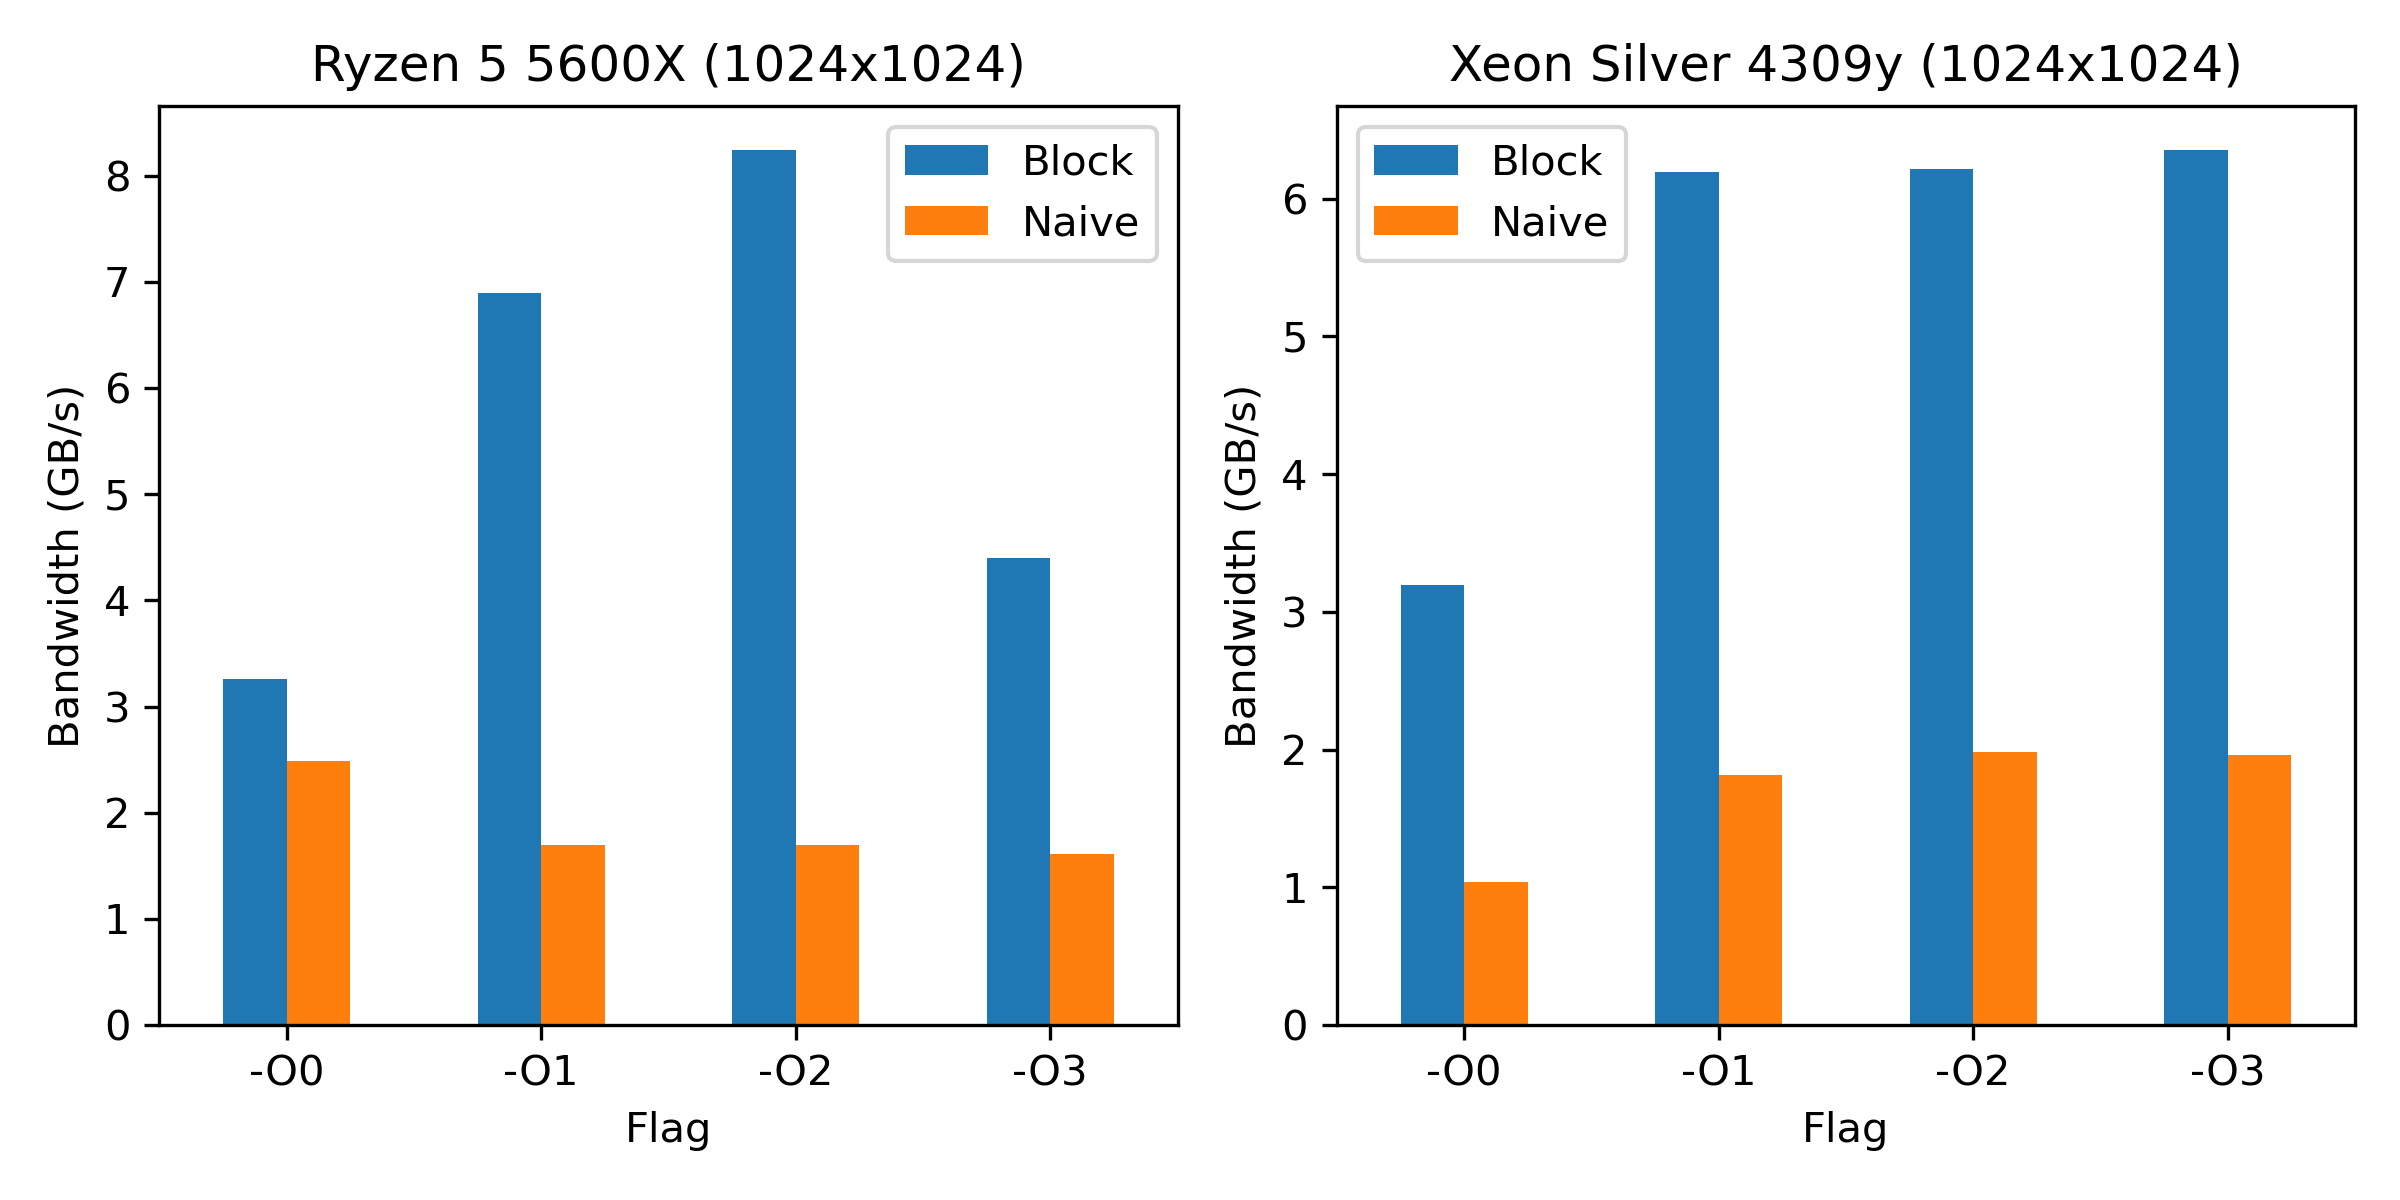
\includegraphics[width=0.85\textwidth]{report/img/block_vs_naive.png}
    \caption{Comparison of the blocked algorithm against the na\"{i}ve algorithm}
    \label{fig:blocked_comparison}
\end{figure*}
\begin{table}[h]
    \centering
    \begin{tabular}{|c|c|c|c|}
        \hline
        \multicolumn{4}{|c|}{\textbf{Ryzen 5 5600X}} \\ 
        \hline
        \textbf{Algorithm} & \textbf{Dimension} & \textbf{I1 m.r.} & \textbf{D1 m.r}. \\ \hline
        Na\"{i}ve & 1024        & 0.00\%       & 4.0\%        \\ \hline
        Blocked  & 1024        & 0.00\%       & 1.4\%        \\ \hline
    \end{tabular}
    \hspace{2em}
    \begin{tabular}{|c|c|c|c|}
        \hline
        \multicolumn{4}{|c|}{\textbf{Xeon 4309y}} \\ 
        \hline
        \textbf{Algorithm} & \textbf{Dimension} & \textbf{I1 m.r.} & \textbf{D1 m.r}. \\ \hline
        Na\"{i}ve & 1024        & 0.01\%       & 3.7\%        \\ \hline
        Blocked  & 1024        & 0.00\%       & 1.0\%        \\ \hline
    \end{tabular}
    \caption{Comparison of the cache miss rate between the na\"{i}ve and the blocked algorithm, \texttt{-O3}}
    \label{tab:blocked_cache_miss}
\end{table}
\section{Conclusion}
To conclude, if provided with an adequate block size, the blocked algorithm is able to achieve an higher effective bandwidth than the na\"{i}ve one.
These results are concordant with the outcomes of the cache analysis. \\
A future direction to further improve the performance could be to parallelize the algorithms. A possible solution could ideally employ the usage of one thread 
for each cell of the matrix. Of course, this approach would require a high number of threads, therefore being impractical for large matrices. Instead, a better solution 
could be to divide the matrix into blocks and assign a thread to each of them.
\newpage
\twocolumn[
\begin{center}
    \textbf{\huge Part 2: CUDA Implementation}
\end{center}
]
\newpage
\section{CUDA Algorithms} \label{algorithms}
During this section, the three proposed algorithms are going to be introduced along with their pseudocode.
For all the implementations, the kernel configuration has been calculated as follows: \\

dim3(TILE\_DIM, TILE\_DIM, 1) \\

dim3(side / TILE\_DIM, side / TILE\_DIM, 1)
\subsection{Na\"{i}ve Transposition}
In the \textit{NaiveTranspose} algorithm, the element at position $[row][col]$ of the source matrix is read and written into the destination matrix at position $[col][row]$.
Note that while the accesses to the $src$ matrix are coalesced, the accesses to the $dst$ matrix are not.
Indeed, the write operations to $dst$ have a stride equal to the width of the matrix.
\begin{algorithm}
    \caption{Naive Matrix Transposition}
    \begin{algorithmic}[1]
        \Procedure{NaiveTranspose}{$src, dst, width$}
            \State $row \gets blockIdx.x \times blockDim.x + threadIdx.x$
            \State $col \gets blockIdx.y \times blockDim.y + threadIdx.y$
            \If{$row \le width \; \&\& \; col \le width$}
                \State $dst[row \times width + col] = src[col \times width + row]$
            \EndIf
        \EndProcedure
    \end{algorithmic}
\end{algorithm}
\subsection{Transposition with Coalesced Memory}
The transposition with coalesced memory exploits the usage of the shared memory to store a tile of the matrix,
avoiding the large strides through the global memory. \\
A downside of this approach is that the usage of shared memory could lead to memory bank conflicts.
\begin{algorithm}
    \caption{Matrix Transpose with Shared Memory}
    \begin{algorithmic}[1]
        \Procedure{Tr\_Coalesced}{$src, dst, width$}
            \State $tile [TILE\_DIM][TILE\_DIM]$
            \State $row \gets blockIdx.x \times TILE\_DIM + threadIdx.x$
            \State $col \gets blockIdx.y \times TILE\_DIM + threadIdx.y$
            \If{$row \le width \; \&\& \; col \le width$} \Comment copy to shared memory
                \State $tile[tIdx.y][tIdx.x] = src[col \times width + row]$
            \EndIf
            \State $\_\_syncthreads()$
            \State $row \gets blockIdx.x \times TILE\_DIM + threadIdx.x$
            \State $col \gets blockIdx.y \times TILE\_DIM + threadIdx.y$
            \If{$row \le width \; \&\& \; col \le width$}
                \State $dst[col \times width + row] = tile[tIdx.y][tIdx.x]$
            \EndIf
        \EndProcedure
    \end{algorithmic}
\end{algorithm}
\subsection{Transposition with Coalesced Memory and No Bank Conflicts}
As mentioned above, a wrong access pattern to the shared memory could result in bank conflicts, which can slow down the execution
of the kernel. To avoid this conflict, the shared memory can be padded with an additional column.
\begin{algorithm}
    \caption{Matrix Transpose with Shared Memory with no Bank Conflicts}
    \begin{algorithmic}[1]
        \Procedure{Tr\_Coalesced}{$src, dst, width$}
            \State $tile [TILE\_DIM][TILE\_DIM + 1]$
            \State $row \gets blockIdx.x \times TILE\_DIM + threadIdx.x$
            \State $col \gets blockIdx.y \times TILE\_DIM + threadIdx.y$
            \If{$row \le width \; \&\& \; col \le width$} \Comment copy to shared memory
                \State $tile[tIdx.y][tIdx.x] = src[col \times width + row]$
            \EndIf
            \State $\_\_syncthreads()$
            \State $row \gets blockIdx.x \times TILE\_DIM + threadIdx.x$
            \State $col \gets blockIdx.y \times TILE\_DIM + threadIdx.y$
            \If{$row \le width \; \&\& \; col \le width$}
                \State $dst[col \times width + row] = tile[tIdx.y][tIdx.x]$
            \EndIf
        \EndProcedure
    \end{algorithmic}
\end{algorithm}
\section{Results} \label{results}
The bandwidth measurements have been performed on the NVIDIA A30 mentioned 
in section \ref{hardware}. The code was compiled with CUDA 12.2. \\
The peak bandwidth used for comparison has been retrieved using the \textit{cudaDeviceProp} structure \cite{nvidia:cudaDeviceProp} and
the obtained value is 933.1 GB/s. 

To evaluate the performance, the algorithms have been tested using various dimensions of the matrix ($256 \times 256$ to $4096 \times 4096$) and
the execution of the kernels has been repeated 100 times to improve the accuracy of the measurements.
Moreover, the kernel configuration has been set accordingly as stated in section \ref{algorithms}, using a block size of $16 \times 16$.
As depicted in figure \ref{fig:algorithm_comparison}, due to the use of the shared memory, both coalesced algorithms outperform the na\"{i}ve one.
\begin{figure}
    \centering
    % 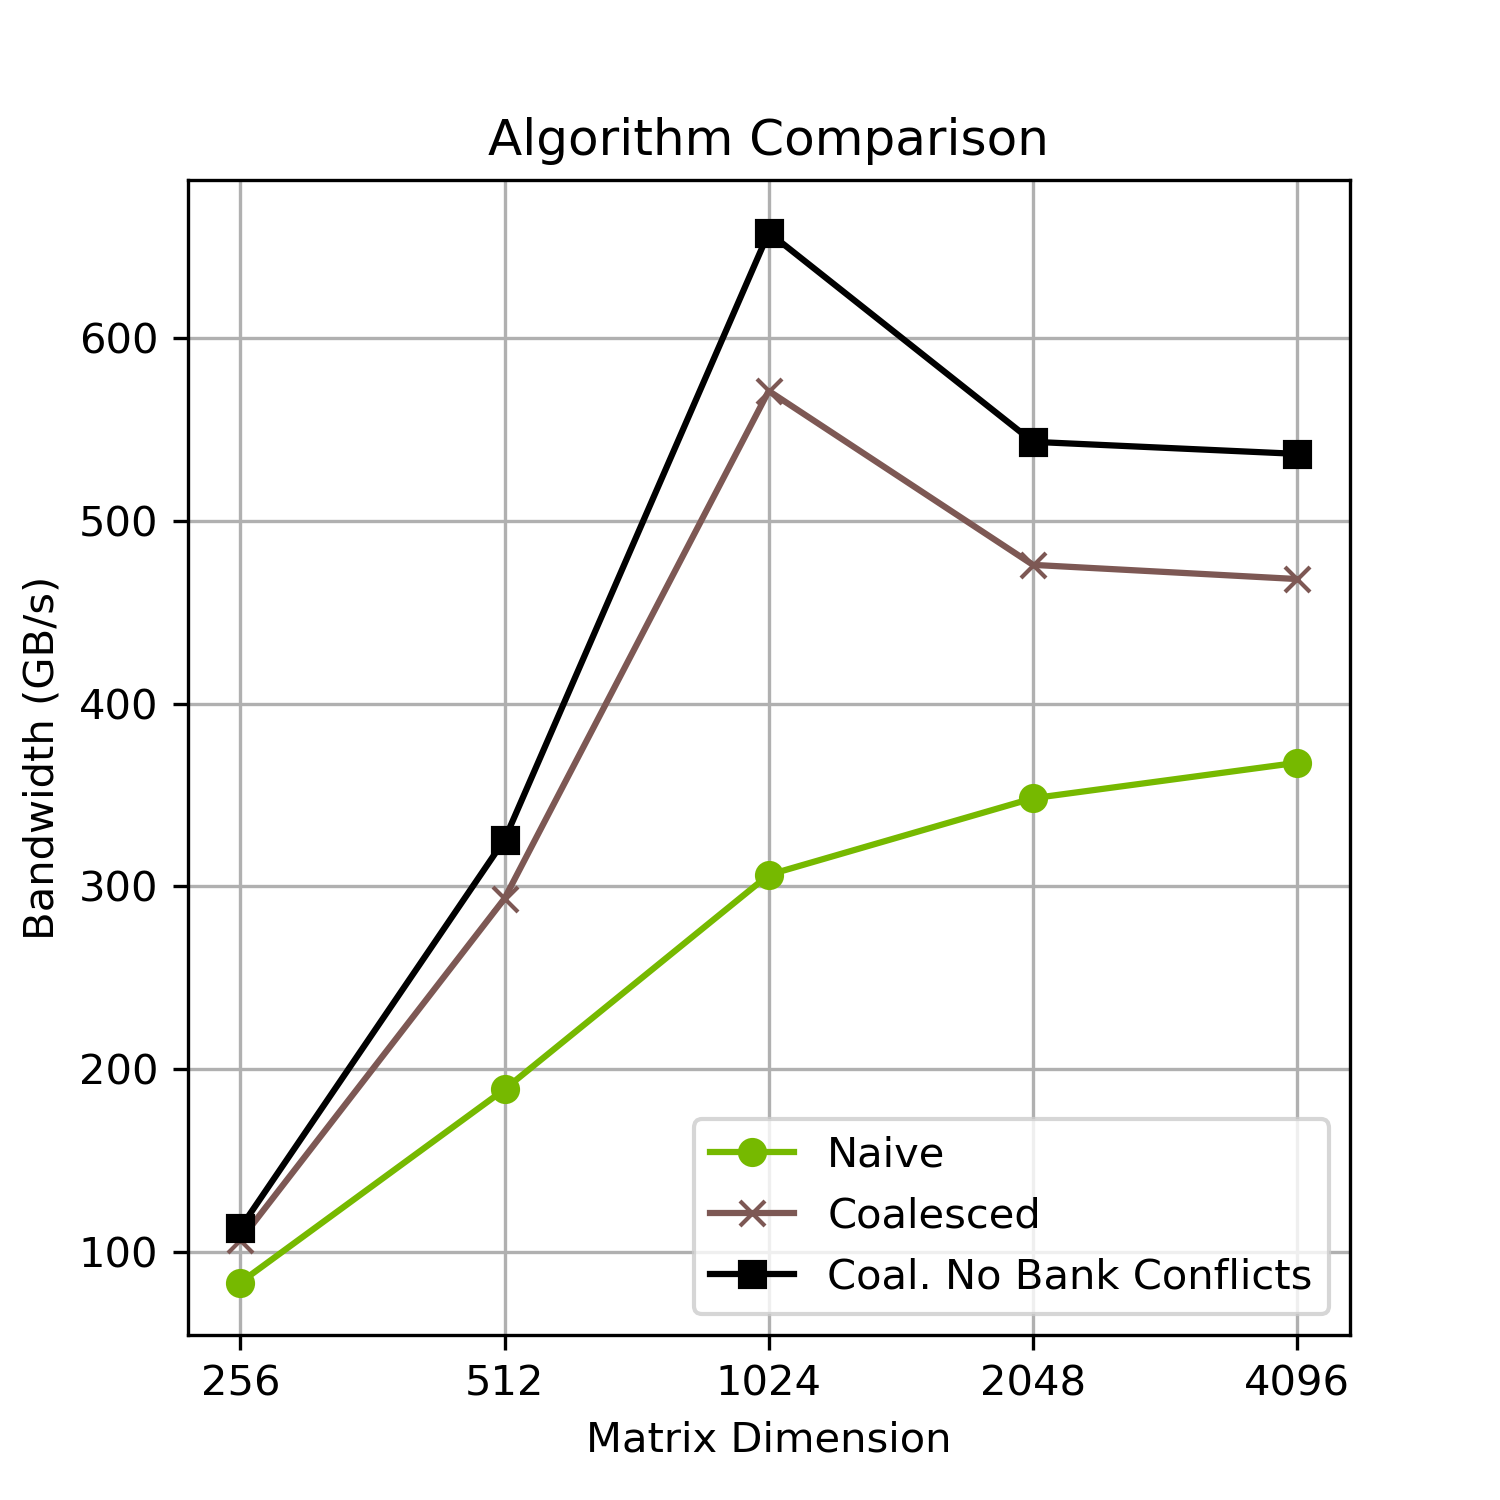
\includegraphics[width=0.55\textwidth]{report/img/algorithm_comparison.png}
    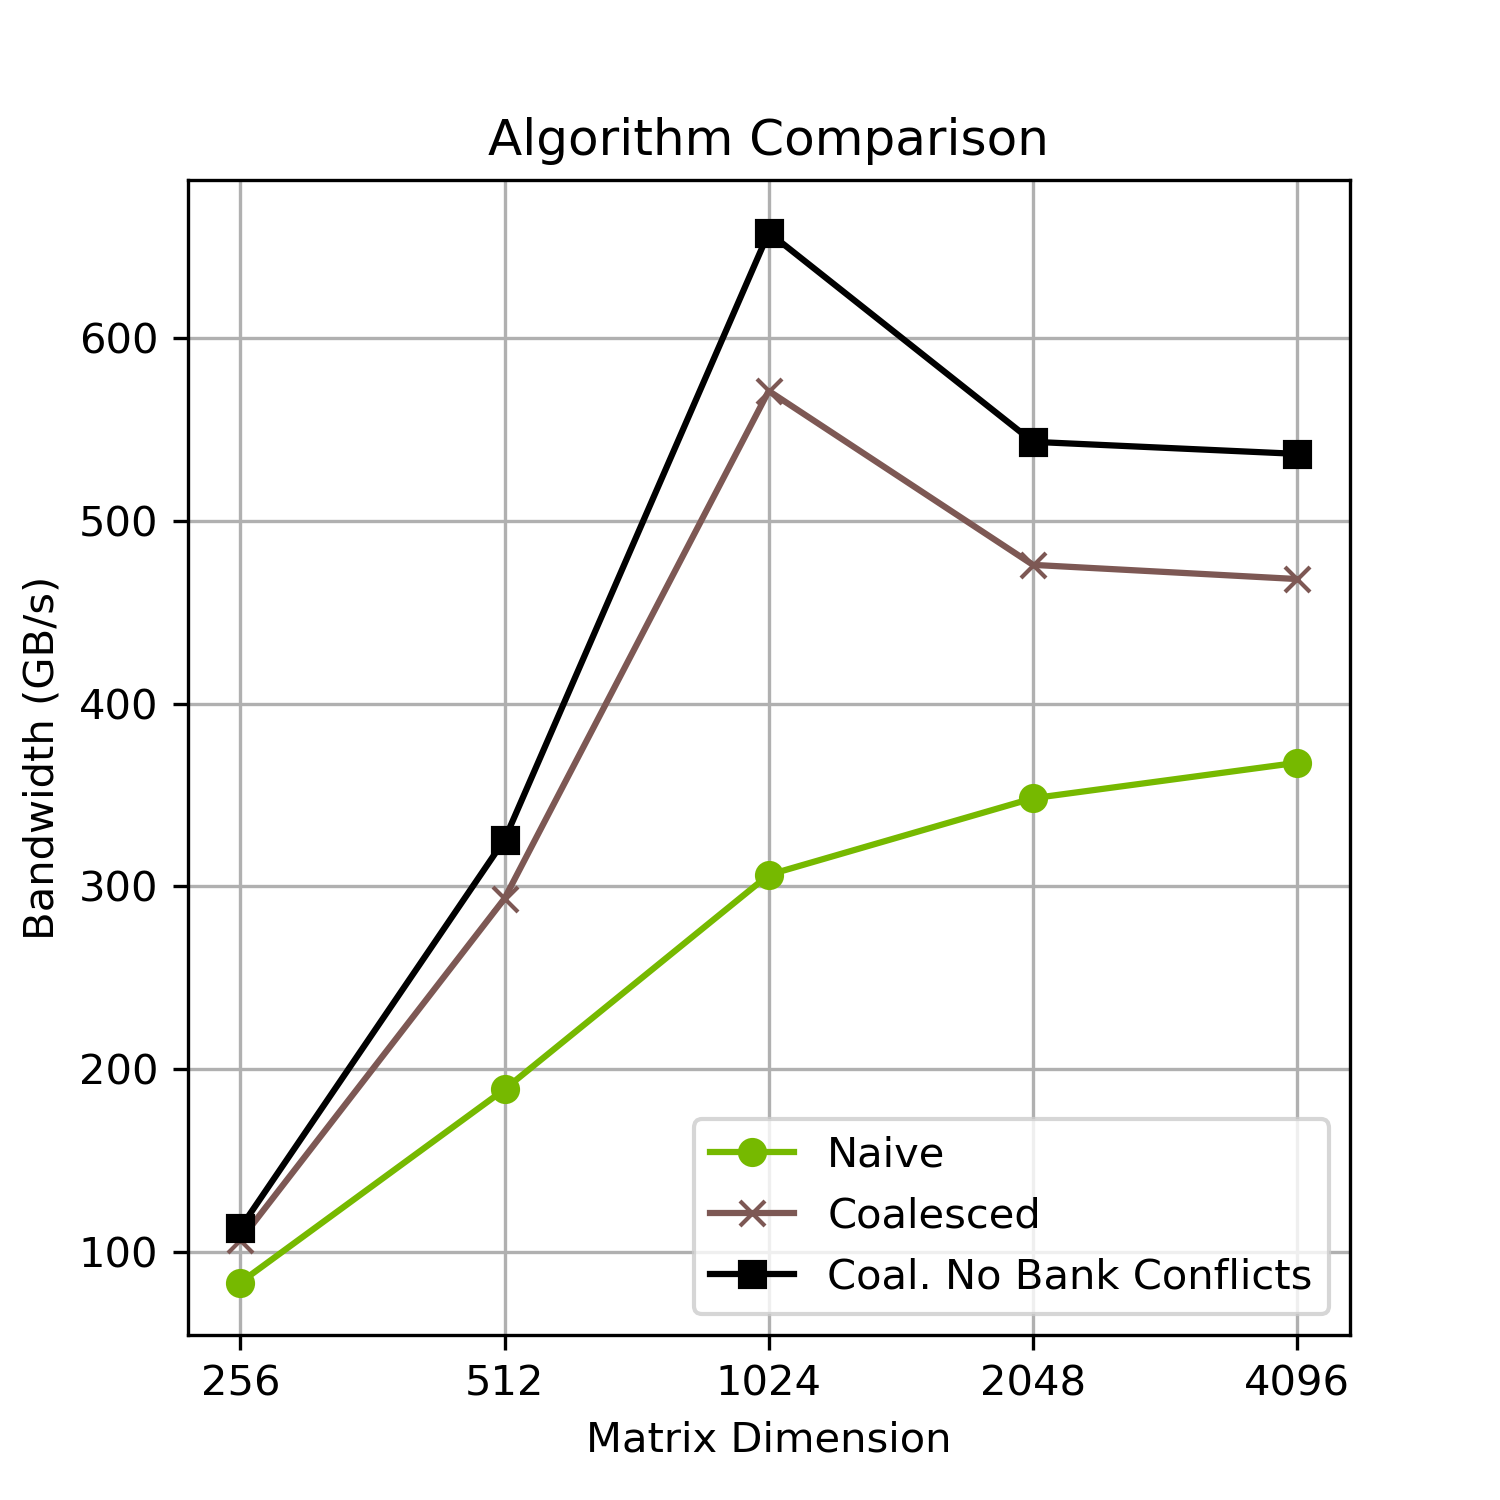
\includegraphics[width=\columnwidth]{report/img/algorithm_comparison.png}
    \caption{Comparison of the different algorithms}
    \label{fig:algorithm_comparison}
\end{figure}

Additionally, an analysis has been conducted to evaluate the performance of the algorithms with respect to different block sizes.
The dimension of the matrix has been set to $1024 \times 1024$.\\
In figure \ref{fig:tile_comparison}, the outcome shows that the $16 \times 16$ block size is the most efficient for all the algorithm.
With a block size of $32 \times 32$ the behavior is more interesting.
In particular, the algorithm with no bank conflicts is not influenced by its size, while the simple coleasced algorithm shows a 
significant decrease in the performance. This is probably due to a high number of bank conflicts, resulting in a lot of accesses to the 
shared memory that need to be serialized. Even the na\"{i}ve algorithm drops in performance, likely because of the high number of accesses
to the global memory.
\begin{figure}
    \centering
    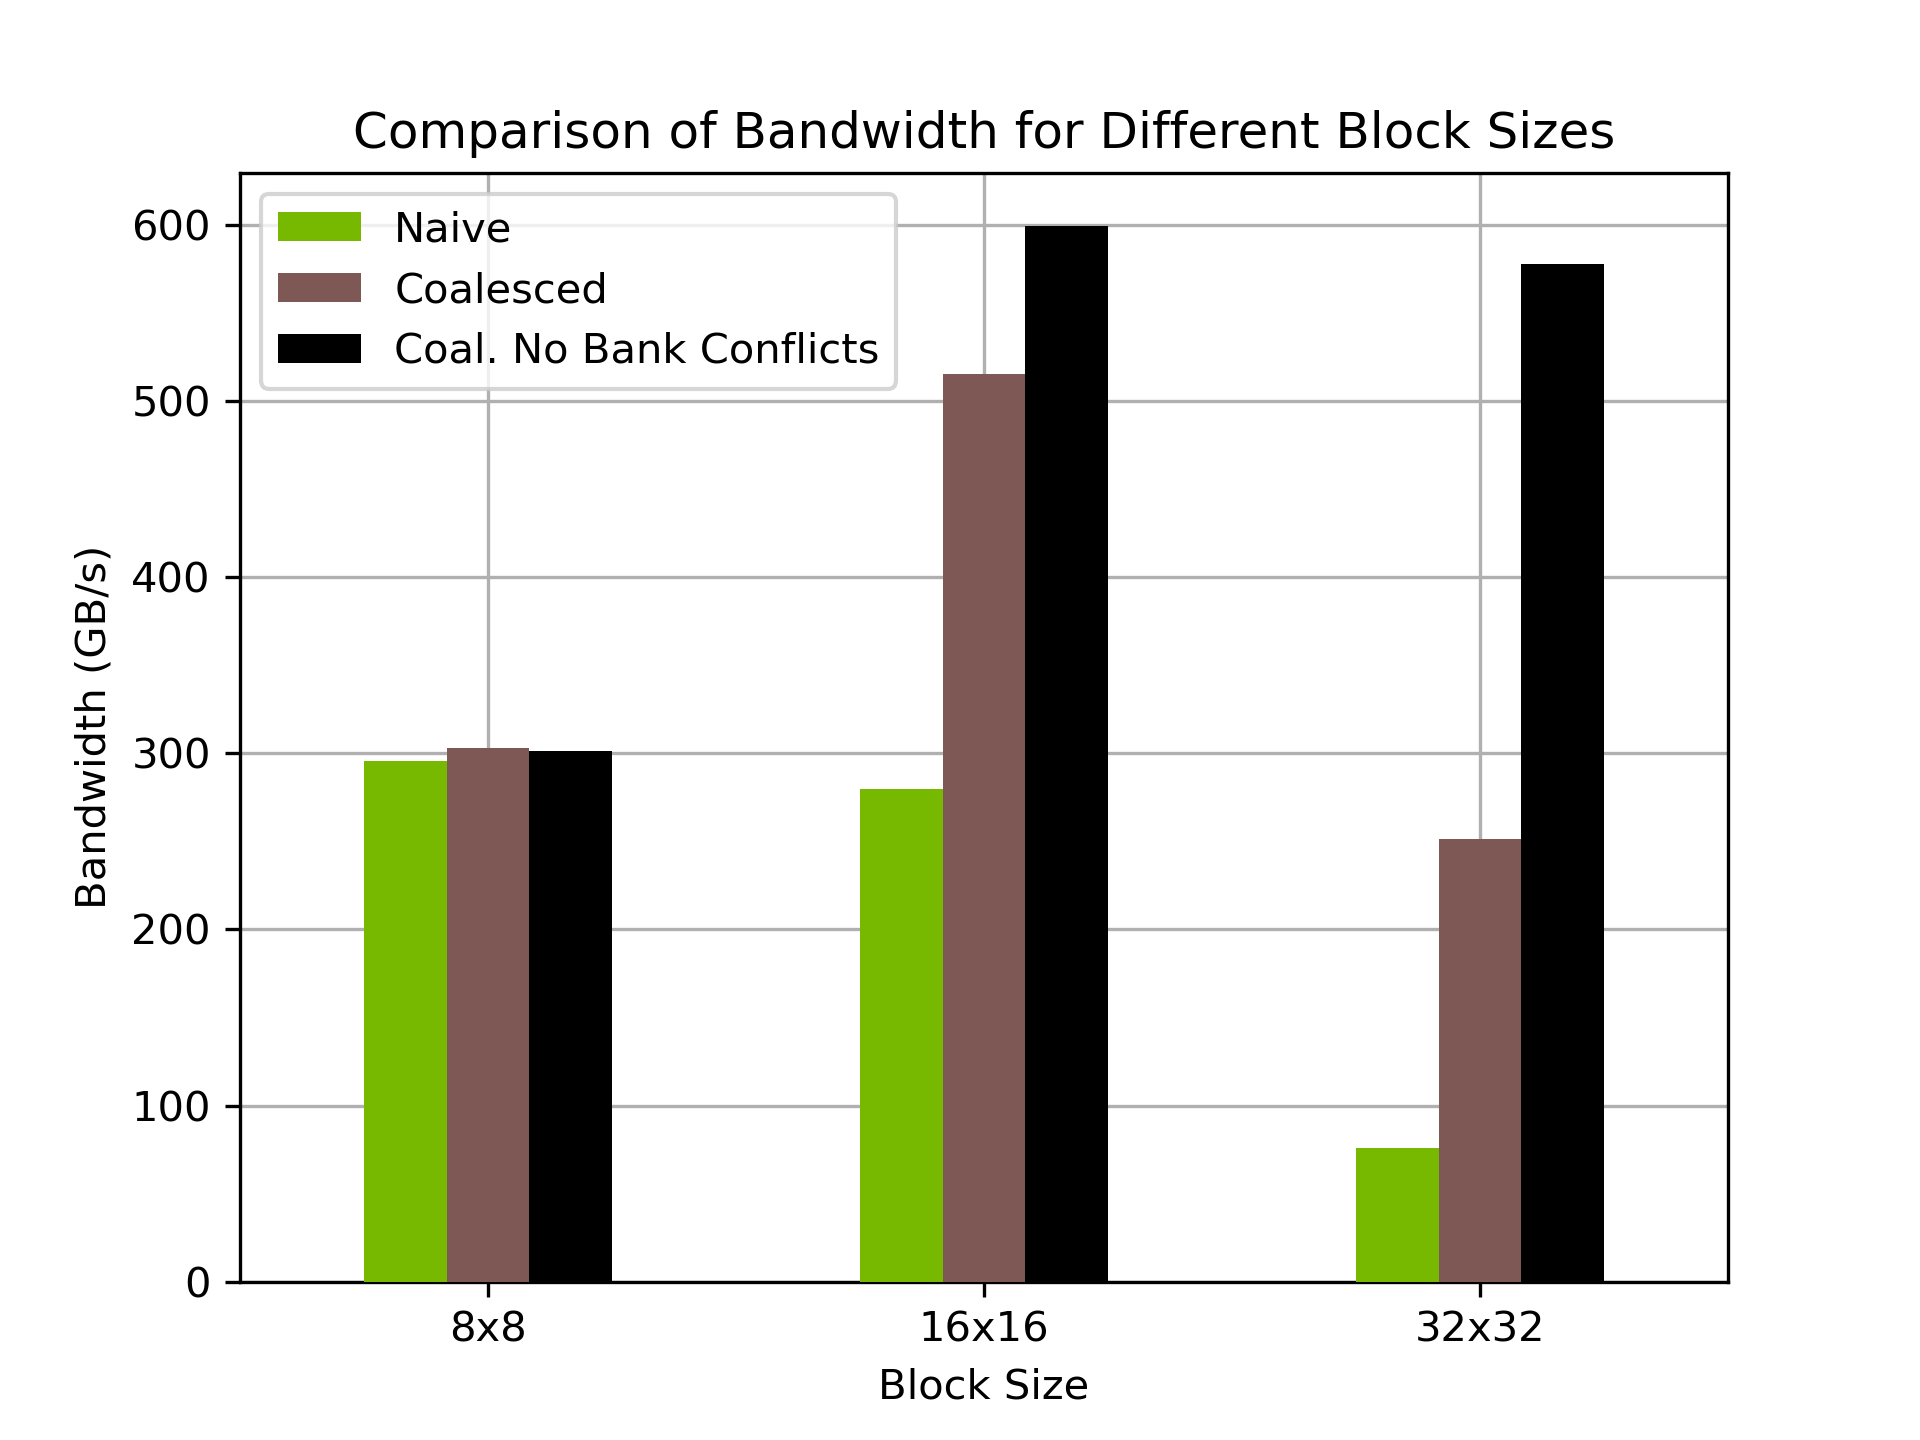
\includegraphics[width=0.55\textwidth]{report/img/tile_comparison.png}
    \caption{Comparison of the different block sizes}
    \label{fig:tile_comparison}
\end{figure}
\section{Conclusion}
To wrap up, three kernels - that represent different approaches to the matrix transposition problem - have been implemented.
This work showed how to exploit the shared memory to coalesce the accesses to the global memory, attempting to enhance the performances.\\
From the previous results (section \ref{results}), we can conclude that both coalesced algorithms benefit from the shared memory, achieving a 
better effective bandwidth than the na\"{i}ve one. Also, the block size plays an important role in tuning the performance.

Coming towards the end, it is worth to mention the speed up gain with respect to the CPU implementation, discussed in the first homework. Although some small matrices are faster to transpose
on the CPU, the GPU is definitely able to surmount the CPU when dealing with larger matrices.
Despite that, there's still room for improvement. Indeed, the algorithms could be further optimized by leveraging
\textit{Warp-level primitives} for efficient inter-thread communication.
Lastly, since the most recent generations of GPU are equipped with \textit{tensor cores}, a possible future direction could be to exploit 
them to achieve better performances.
\clearpage
\bibliographystyle{plain}
\bibliography{references}
\end{document}

